\documentclass[11pt,twoside]{report}
\usepackage{preamble}
\graphicspath{{../img/ch3/}}
\setcounter{chapter}{2}


\begin{document}

\chapter{The Behaviour of Zebrafish in 2D}
\label{chapter:fish_2d}

The vast majority of the collective behaviour of fish were performed in a quasi--2D environment, where the fish were confined in a shallow water tank. The motions of the fish can be captured by digital cameras and analysed by tracking softwares.

\section{Introduction}

In this chapter we will explore the behaviour of zebrafish in a quasi two dimensional environment, by placing them in very shallow water pool. The deliberate choice of this confinement, was based on technical conveniences. The movement of fish in 2D can be captured by a conventional camera, while their 3D movements are difficult to record.

Even though the videos of a group of moving fish can be recorded easily, there are still technique challenges to extract the behaviour out of the experimental record. The difficult task is to identify of individual fish in a group.


\section{Methods}

This section will present my way to attack the technical challenges, for the 2D behaviour of zebrafish. The necessary methods to track a group of fish in a video will be introduced, and the ideas can be applied beyond animal tracking, for instance the analysing of 2D colloidal experiments.

\subsection{Image Processing}
\label{section:image_process}

To get useful information out of the image, we want to transform the video, where the fish appear as a dark spot, into a better representation. Ideally, the processed image should be a collection of delta functions, where the pixel intensity in the centres of each individual fish is maximum, and the pixel intensities are zero everywhere else. Even though it is possible to construct such transformation directly with machine learning based approaches \cite{newby2018}, it is still not a straightforward and easy task. Traditional image processing methods such as thresholding, blurring, and morphological operations were still applied a lot in this project. As a result, I get a video where each fish have high pixel intensity values and the background intensity values are zero. Figure \ref{fig:2d_process} illustrate the result of the transformation. On the left side is the video recorded during the experiment, and the central image is the ``foreground'' after the image processing, where the background is removed.

I obtained the foreground videos of the fish with two different steps, the removal of the background and removal of the noises. The background is defined as the temporal average of the image, since the fish are constantly moving while rest of the scene is static. In order to tackle the varying illumination conditions\marginfootnote{
The brightness level fluctuates even I keep the illumination setting unchanged in the laboratory. In a relatively dark ($\sim$20 lux) condition, those fluctuations could not be ignored.
}, I take a running average of a time--window, instead of calculating the overall average. The pixel intensity of the background at time $t$, of pixel $(x, y)$, can be written as

\begin{equation}
I_\mathrm{bg}(t; x, y) = \frac{1}{T} \sum_{\tau=t}^{t+T}{I(\tau; x, y)}
\label{eqBG}
\end{equation}

\noindent where $I(\tau; x, y)$ is the pixel intensity of the video at time $\tau$ in position $(x, y)$, and $T$ is the duration of the window, usually taken as 40 seconds. The difference between the background video and original video yields a foreground video, written as

\begin{equation}
	I_\mathrm{fg}(t; x, y) = I_\mathrm{bg}(t; x, y) - I(t; x, y)
\label{eqFG}
\end{equation}

\noindent and the order of the subtraction ensures the fish, originally appear darker in the video, would be represented by brighter pixels in the foreground video, shown in the centra image in Fig.\ \ref{fig:2d_process}. The subtraction result are often very noisy. To remove the noise, I applied gaussian filter to the foreground image, to smooth the sharp noises. Additionally, I applied the a combination of Otsu (大津) threshold and local gaussian threshold to separate the pixels belonging to the fish and other pixels. The Otsu threshold separate all the pixels into different groups to minimise the inter--group variance of the intensity distribution. LOCAL THRESHOLD.

\begin{SCfigure}
  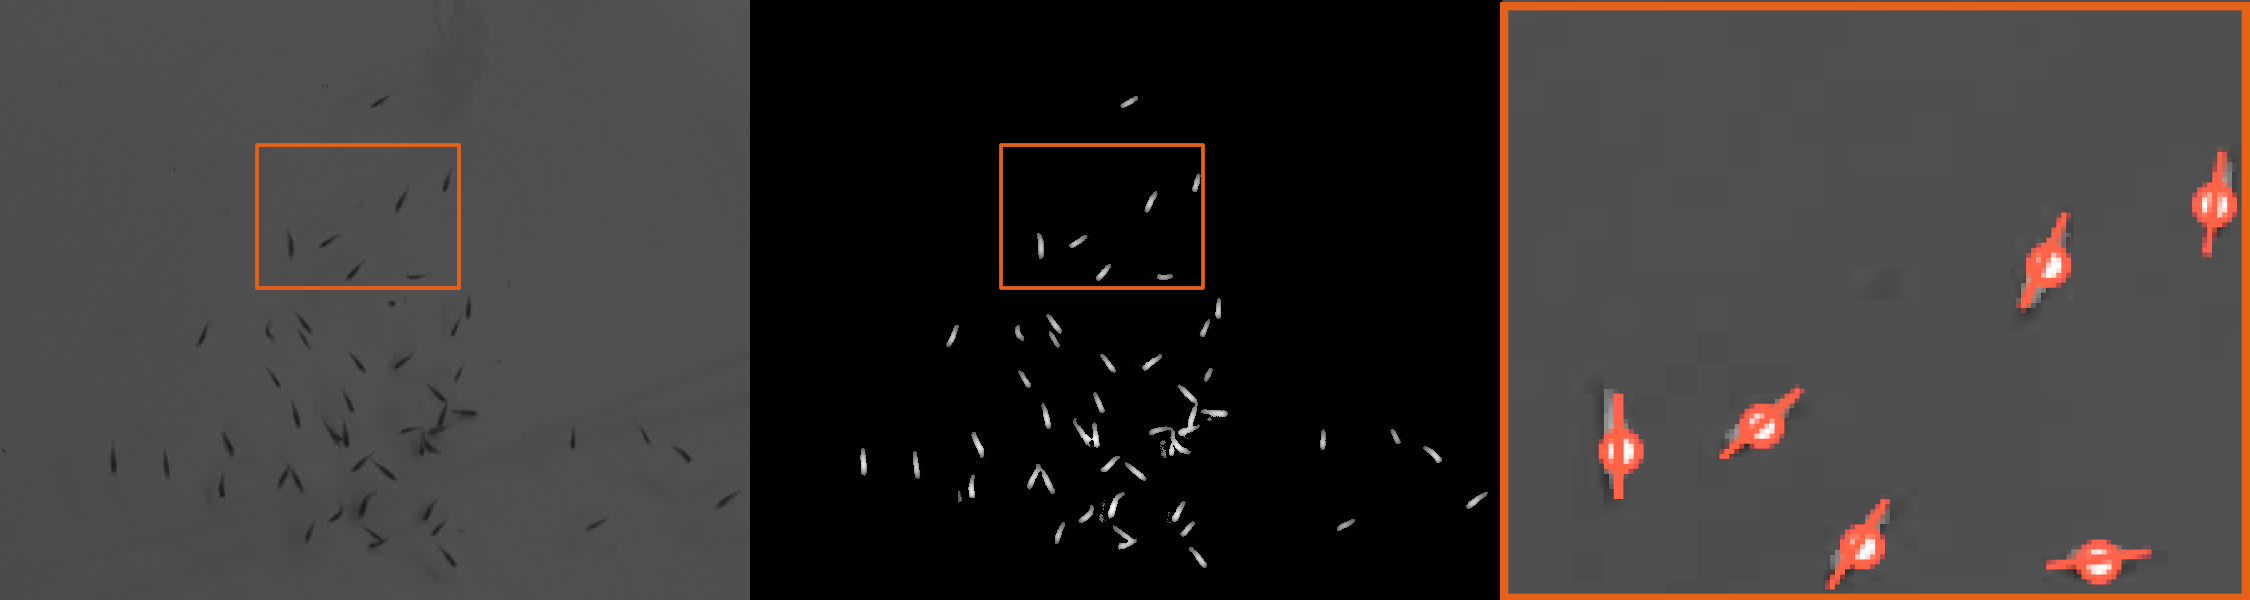
\includegraphics[width=\linewidth,outer]{2d-processing.png}
  \caption{}
  \label{fig:2d_process}
\end{SCfigure}


\subsection{Extracting Features: General Idea}
\label{section:oishi}

From the processed video, it is to possible extract the features
\marginfootnote{
In the computer vision community, people call the locations of objects ``features''. This slightly odd name roots in the 3D reconstruction problem, which will be discussed in the next chapter. Very briefly, we can not recover 3D geometry from the background, like a purely white wall, where all the pixels have the same intensity value. Instead, some ``features'', with intensity gradients, are required\cite{ma2005}. Adapting this naming tradition, the positions of the fish in 2D images will be called ``features''. An alternative name would be the just the ``positions''. However, the selected name stressed the nature of a fish image in the photo: it is a ``feature'' of the photo, but not a (3 dimensional) position of a fish.
}
in each frame that corresponds to the fish. In order to tackle the problem, we employed a method that not only capture the positions, but also the information of the fish orientations and body shapes. The basic idea is to calculate the cross--correlation between the image ($\mathbf{I}$) and a templated fish shape ($\mathbf{T}$), as the local maxima in the result would indicate the presence of a fish, because cross--correlation is a measure of similarity between signals.

For a fixed 2D fish template ($\mathbf{T}(x, y)$), we can rotate it so that it contains $r$ different orientations. Calculating the cross--correlation of all the rotated templates, we can effectively get $r$ different results, and they can be concatenated into a 3D tensor (array), written as $\mathbf{C}(x, y, r)$. The tensor $\mathrm{C}$ can be treated as 3D volumetric image. A local maxima in $\mathbf{C}$, with coordinate $(x_m, y_m, r_m)$, indicates the presence of a fish at location $(x_m, y_m)$, with orientation $r_m$.


In addition, we are free to choose different templates for the fish shape, to capture the different postures. If $s$ different shapes were selected as templates, all of which were rotated into $r$ different orientations, then there will be $s \times r$ different templates. The cross-correlation of these templates with the image would yield a 4D tensor that can be shaped into $\mathbf{C}(x, y, r, s)$. A local maxima in the tensor, with coordinate $(x_m, y_m, r_m, s_m)$, represents a fish located at $(x_m, y_m)$, whose posture is like the $s$th template, with orientation $r_m$.


In summary, the cross--correlation between the image and the many templates yields a 4D tensor. This will be helpful for dealing with ``dense'' system, where the fish constantly overlap with each other. For the dense system, different fish will be separated into different regions in the shape--rotation space. For example, the overlapped fish pair in Fig.\ \ref{fig:fish_cross} was correctly labelled, by calculating the local maxima in the 4D tensor.


\begin{SCfigure}
  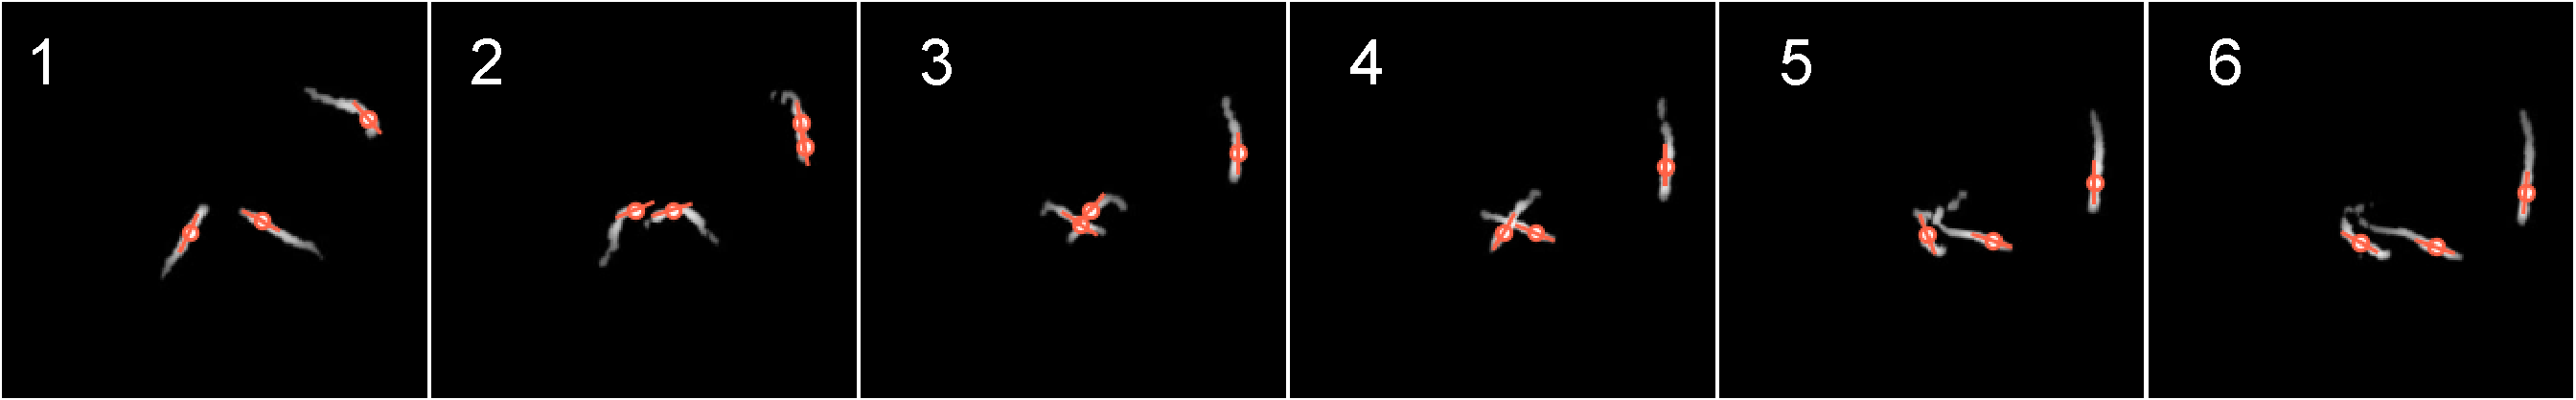
\includegraphics[width=\linewidth,outer]{cross-resolve}
  \caption{The movement of 3 fish in 6 successive frames. The crossed fish pair correctly labelled by the oishi feature detection algorithm.}
  \label{fig:fish_cross}
\end{SCfigure}


\subsection{Extracting Features: Find Templates}
\label{section:oishi_template}

\subsection{Extracting Features: Speeding up}
\label{section:oishi_optimise}

The mapping from the image to the tensor, $\mathbf{I}(x, y) \rightarrow \mathbf{C}(x, y, r, s)$, can be viewed as the Hough transformation, where the fish geometry is described by $(x, y, r, s)$. Like conventional Hough transformation, our method requires large amount of calculation while scanning the entire 4D parameter space. The speed can be significantly increased if the calculation were only performed on ``promising'' positions were a fish is likely to appear, and these positions corresponds to the local intensity maxima in the foreground image $I_\text{fg}$, defined in Eq.\ (\ref{eqFG}).

\section{General Methods for nD data}

This section will introduce the algorithms that are used for both 2D experiments and the 3D analysis of fish behaviours, which would be discussed in the next chapter.

\subsection{Linking Positions to Trajectories}
\label{section:link}

With the positions of all the fish, one can study the \emph{structure} of the fish group. However, extra work needed to be carried out in order to obtain the \emph{dynamic} of the system. Because the velocities of each fish is needed to calculate the dynamical quantities like the spatial/temporal velocity correlation function, which is used to extract the correlation length and the leadership relationship. To get the velocities, it is necessary to link the positions, at different time points, into trajectories. The concept is illustrated in.

% words and figure to illustrate a linking procedure.

The linking procedure requires a prior knowledge of the dynamic of the system under study. For example, the dynamic of colloidal particles is known to be Brownian, whose.

% introduce the CG linking procedure.

However, the situation for the fish is a bit different: we don't really know the dynamic of the fish, hence the cost function to minimise in the linking procedure is a bit unclear.

To tackle the situation, to my best knowledge, one can start with very simple assumptions. One possible choice is the constant speed.

% introduce Ouellette's paper.

Implementing the algorithm, I obtained some very short trajectory segments. These segments can be extended further following

% introduce Xu's idea and the global optimisation procedure.

Practically, enumerating all the possible linking choices can take a very long time. So

% talk about the heuristic to restrain dt dx.

Pass


\subsection{Removing Overlapped Particles}
\label{section:overlap}

I used linear programming method to remove overlapped coordinates. The overlap happened if different parts of the fish matched different kernels.

Supposing there are $N$ particles in total, and we wish to find $K$ non--overlapping particles, where each particle has an uncertainty value of $e_i$. The task can be written as a linear programming problem with quadratic constrains as follows:

\begin{equation}
\begin{aligned}
	\textrm{Minimize} && \sum_i{e_i x_i} \\
	\textrm{Subject to} && d_{12} x_1 x_2 \le \sigma \\
	&& d_{13} x_1 x_3 \le \sigma \\
	&& \vdots  \\
	&& d_{ij} x_i x_j \le \sigma \\
	&& \sum_i{x_i} = K
\end{aligned}
\end{equation}

\noindent where $d_{ij}$ is the distance between particle $i$ and $j$, $\sigma$ is the diameter of the non--overlapping hard core of each particle, and $K$ is the total number of particles. The solution to above cost function and constrains can be effectively solved by the CPLEX optimisation package. (SITE IBM).\marginfootnote{As a recent development, IBM announced a faster version of CPLEX using the deep neural network to perform the same optimisation task.}

An alternative choice is to apply a greedy algorithm, to always remove the worst match until there is no overlap. The greedy algorithm is much easier to implement, and can sometimes find good solutions. However, the linear programming method will find the global minimum of the cost, therefore being selected in my study.

The overlapping resolve method introduced in this subsection can be extended beyond tracking animals. In fact, it can be very helpful to refine the particle tracking result for colloidal experiments, where the traditional algorithm might give overlapping coordinates because of intensity noises. In the colloidal experiment, the error term can be the inverse of the fluorescent intensity (to favour brighter centres) or the response to a kernel function (to favour a particular shape).

\section{Possible Improvements for the Methods}

This section included some possible ideals to improve the methods mentioned above. Due to the limited time of the PhD project I did not fully explored the ideas below. However, preliminary results suggests that these ideals are worth being further explored.

\subsection{Convolution Neural Network}
\label{section:cnn}

There are two steps in the image processing that can be improved in the image processing pipeline. The first one is the removal of background. In my current method, I calculated a rolling average of the entire video. The window size of the averaging operation is set by the user, which is very difficult to optimise because the video processing typically takes hours to finish. Practically, a rule-of-thumb number (600 frames) was applied. However, the fish in the video are very distinct from their background, and it is an easy task for people to spot the fish in a static image. This suggests a static image contains enough information to distinguish the foreground (fish) and background (tank). 

The neural network is very suitable for extracting the needed information in our case. Developed in the 1980s and revived very recently (2010).

\subsection{Hierarchical Shape Matching}
\label{section:hierarchical_shape}

In the current method, the shape templates were generated from clustering the features in a low--dimensional space.

\subsection{Recursive Neural Network}
\label{section:rnn}

The linking problem might be better handled with a RNN.

\section{Result}

In this section I wil

\subsection{The behaviour of 1 fish}
\label{section:fish_1_2d}

\subsection{The behaviour of 2 fish}
\label{section:fish_2_2d}

\subsection{The behaviour of 3 fish}
\label{section:fish_3_2d}

\subsection{The behaviour of Many fish}
\label{section:fish_many_2d}

\end{document}